\documentclass[a4paper]{article}
\usepackage[latin1]{inputenc}
\usepackage[english]{babel}
\usepackage{graphicx}
\usepackage[linewidth=1pt]{mdframed}
\usepackage{tikz-qtree}
\usepackage{algorithm}
\usepackage{algorithmic}
\usepackage{amsmath}
\usepackage{url}
\usepackage{caption}
\usepackage{subcaption}
\usepackage[margin=2cm]{geometry}

\title{iMSG: Guiding language evolution by the need to express}
\author{Michael Cabot\\6047262 \and Sander Latour\\5743044}

\begin{document}
\maketitle
\section{Introduction}
\cite{zuidema2003poverty} \cite{batali1999negotiation}
In language learning, communication between a parent and a child typically starts with a semantic message (from now on referred to as the \emph{intention}) that the parent wants to share with the child. In order to communicate the intention, the parent needs to express it into a specific language formalism according to grammar rules known to the parent. The child then receives that expression in combination with the expressed intention. Although many communication happens between a parent and a child where there is not an explicit transfer of the intention, we focus on the part of language learning where the verbalized intention is somehow pointed out in other ways than verbal language (e.g. by ensuring a similar observation). Based on earlier communications together with the current one, the child attempts to induce structural grammar rules on how to parse and generate expressions. From all grammars that could be responsible for the observations the child constructs the one that was easiest to learn according to its learning algorithm.  In the next iteration the child becomes the parent who in turn communicates intentions to a new child. With each iteration the grammar becomes more structured and thus easier to learn for the child in the next iteration. 

Progress in the field of iterated learning has been made by \cite{zuidema2003poverty}. Here the child exploits regularities in the strings it receives to construct a context-free-grammar (CFG). Once the child becomes the parent it generates strings from its grammar which are send to a new child. Zuidema's results show that over time the parent's grammar becomes easier to learn, contains fewer rules and decreases in its expressiveness, i.e. the amount of strings recognized by the grammar. Noticeable is that Zuidema enforces a minimal expressiveness of the grammar by checking if its expressiveness $E_G$ is smaller than a predefined minimal expressiveness $E$. If this is the case, $E - E_G$ new random strings are incorporated into the grammar. Without this constraint, the grammar would converge to a single context-free rule. We believe that the necessity to express a certain set of intentions will take care of the decreasing expressiveness of the grammar in a more natural way. The hypothesis is that by providing the parent with a list of intentions it needs to express, the iterated language evolution will optimize the language without reducing it to triviality. In order to test this hypothesis, this paper presents a semantic-driven iterated language learning framework based on both the work of \cite{zuidema2003poverty} on language evolution and the work of \cite{batali1999negotiation} on inducing semantic grammars from observations.

%\textbf{TODO: language evolution, iterative process between parent and child. progress made, especially by zuidema in reducing number of restrictions and assumptions. however problem in ever-decreasing grammar size}

This paper is structured as follows. Section \ref{sec:system_overview} describes the system that was build. In section \ref{sec:experiments}, the experiments are described that were conducted to test the hypothesis. The results of these experiments are discussed in sections \ref{sec:results} and \ref{sec:discussion}. Section \ref{sec:conclusion} summarizes the results in this paper.

%\section{Related work}
%explain batali
%explain zuidema
%explain how this paper differs
\section{Notation and Vocabulary}
% TODO batali gebruikt fragments, wij CFG rules
\begin{description}
    \item[formula] A formula $f$ consists of a predicate, denoted as $pred(f)$, and zero or more arguments, denoted as $args(f)$. The number of arguments is defined by the type of the formula, denoted by $type(f)$, which in this paper is either \verb|PropertyFormula| or \verb|RelationFormula| with one and two arguments respectively. For example, the formula \verb|(snake, 1)| has $pred($\verb|(snake,1)|$)$ = \verb|snake|, $args($\verb|(snake,1)|$)$ = $[1]$ and $type($\verb|(snake, 1)|$)$ = \verb|ProperyFormula|.
    \item[intention] An intention is a set of formulas that as a whole contains some semantic message. For example, an intention could contain \verb|[(tweety, 1), (see, 1, 2), (pussycat, 2)]| to express that tweety sees a pussycat. Intentions can be combined with other intentions by merging the sets.
    \item[rule] A rule $r$ is similar to an unnormalized PCFG rule. The left-hand-side of the rule, denoted by $lhs(r)$, is an intention. The right-hand-side of the rule, denoted as $rhs(r)$, is a set of intentions that together combine into $lhs(r)$. Linked to the rule is the cost of using the rule, denoted by $cost(r)$, which inversely relates to the probability of that rule being used.
    \item[argument mapping] For each intention $m$ in $rhs(r)$ there is an argument mapping that describes the transformation between the arguments of $m$'s formulas and the corresponding formulas in $lhs(r)$. For example, in figure \ref{fig:rule} the argument of [(tweety, 1)] remains the same while the arguments of [(see, 1, 2),  (pussycat, 2)] are inverted.
    \item[lexical rule] A lexical PCFG rule $r_l$ differs from normal rules in that the left-hand-side contains only one formula and $rhs(r_l)$ is a string of characters (i.e. a word). In this paper, $lhs(r_l)$ will for lexical rules denote the only formula in the left-hand-side. As a result, $type(lhs(r_l))$ will denote the type of the single formula in $lhs(r_l)$.
    \item[grammar] A grammar $G$ consists of all rules and lexical rules. The grammar $G_l$ is a subset of $G$ and contains only the lexical rules from $G$.
% argument mapping
\end{description}

\begin{figure}[h!]
\centering
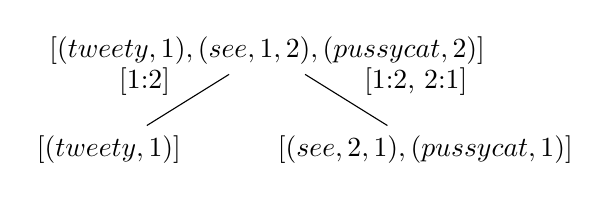
\begin{tikzpicture}[
   level distance=1.25cm,sibling distance=1cm,
   edge from parent path={(\tikzparentnode) -- (\tikzchildnode)}]
\Tree
[.\text{$[(tweety, 1), (see, 1, 2), (pussycat, 2)]$}
    \edge node[auto=right,pos=.6] {[1:2]};
    [.\text{$[(tweety, 1)]$}
        ]
    \edge node[auto=left,pos=.6] {[1:2, 2:1]};
    [.\text{$[(see, 2, 1), (pussycat, 1)]$} 
        ]
]
\end{tikzpicture}
\caption{A context-free rule with intentions and argument mappings.}
\label{fig:rule}
\end{figure}

\section{System overview}
\label{sec:system_overview}
In order to explore the effect of this paper's approach and the validaty of the hypothesis, a computer simulation was designed and implemented. The computer simulation consisted of three main parts: \emph{generating intention}, \emph{expressing intention} and \emph{inducing grammar}. These parts will be described in the following sections.
% image depicting the general outline (parent -> child, iterated loop)
\subsection{Generating intention}
\label{ssec:Generating intention}
Three different methods were developed to obtain an intention to express. The first one is simply by taking a uniform random sample from a fixed set of intentions. The other two methos are \emph{predicate sampling} and \emph{template sampling}.
\subsubsection{Predicate sampling}
\label{sec:predicate_sampling}
A variation to having a predefined set of intentions is to only sample from predefined templates. These templates consist of placeholders that specify the type of formulas that can be ingested and the arguments that the formula wil have. For example, the template \verb|[(PropertyFormula, 1), (RelationFormula, 1, 2), (PropertyFormula, 2)]| allows for intentions that contain two properties and a relationship between them. A possible instantiation of this template is \verb|[(snake, 1), (bite, 1, 2), (pig, 2)]|. The templates ensure a certain complexity in the intention, without fully specifying it. The instantiation of the template is done by sampling formula predicates from the grammar that fit the specified type. The probability density function for this sampling is defined by the inverse cost of the lexical rule related to each formula. In order to deal with the situation where the grammar is still small and the amount of existing predicates in the grammar is limited or none, an exploration rate $\epsilon$ is introduced. The exploration rate defines the chance that a uniform sample is drawn from the set of unused (i.e. unknown to the parent) predicates instead of sampling them from the grammar. The instantiation of a template by sampling is described in the following algorithm:
\begin{mdframed}
    \textbf{Procedure 1} \textsc{PredicateSampling}\vspace{0.2cm}\hrule\vspace{0.2cm}
\noindent For each placeholder $t_i$ in template:
\begin{enumerate}
    \item Draw random number $\theta$, where $0 \leq \theta < 1$
    \item Initialize cumulative probability $p \gets 0$
    \item Initialize the set of unused formula predicates $U$ to the predefined set of all possible predicates of $type(t_i)$
    \item Define grammar subset $G_l'$ as $\left\{r \in G_l | type(lhs(r)) = type(t_i)\right\}$
    \item Calculate normalization constant $Z = \sum\limits_{r \in G_l'} \frac{1}{cost(r)}$
    \item For each lexical rule $r_l \in G_l'$:
        \begin{enumerate}
            \item Remove $pred(lhs(r_l))$ from $U$
            \item $p \gets p + \frac{1-\epsilon}{cost(r) \cdot Z}$, where $\epsilon$ is the exploration rate
            \item If $p \geq \theta$ then \textbf{insert} $pred(lhs(r_l))$ and \textbf{return}
        \end{enumerate}
    \item If $U \neq \emptyset$ then \textbf{insert} a random predicate from $U$ and \textbf{return}
    \item $\epsilon \gets 0$
    \item Go to step one
\end{enumerate}
\end{mdframed}
\subsubsection{Template sampling}
\label{ssec:Template sampling}
One set further than predicate sampling in fixed templates, is to also sample the templates from the grammar. The probability density function for templates is inversely related to the sum of the cost of all the rules that instantiate the template in their left-hand-side. Furthermore the probability of a template $t$ is normalized for the number rules needed to construct the instantiation using the normalization term $2 \cdot \left|\left|t\right|\right| - 1$, which is derived by combining the number of lexical rules ($\left|\left|t\right|\right|$) with the number of rules needed in the parse tree to reach the top ($\left|\left|t\right|\right|-1$). In order to deal with the situation where the grammar is still small and the amount of instantiated templates in the grammar is limited or none, the same exploration rate $\epsilon$ is used as in section \ref{sec:predicate_sampling}. Once a template is sampled, it can be instantiated using the earlier described \textsc{PredicateSampling} procedure. The sampling of a template is described in the following algorithm:
\begin{mdframed}
    \textbf{Procedure 2} \textsc{TemplateSampling}\vspace{0.2cm}\hrule\vspace{0.2cm}
\begin{enumerate}
    \item Draw random number $\theta$, where $0 \leq \theta < 1$
    \item Initialize cumulative probability $p \gets 0$
    \item Initialize the set of unused templates $U$ to the predefined set of all possible templates
    \item Calculate normalization constant $Z = \sum_{r \in G} \left[ \frac{1}{cost(r) \cdot 2 \cdot \left|\left|lhs(r)\right|\right| - 1} \right]$
    \item For each rule $r \in G$:
        \begin{enumerate}
            \item Convert the intention $lhs(r)$ to template $t$ by replacing the formula predicates with their type
            \item Remove $t$ from $U$
            \item $p \gets p + \frac{1 - \epsilon}{cost(r) \cdot 2 \cdot \left|\left|lhs(r)\right|\right| - 1}$, where $\epsilon$ is the exploration rate
            \item If $p \geq \theta$ then \textbf{return} $t$
        \end{enumerate}
    \item If $U \neq \emptyset$ then \textbf{return} a random template from $U$
    \item $\epsilon \gets 0$
    \item Go to step one
\end{enumerate}
\end{mdframed}
\subsection{Parent: Expressing intention}
Once an intention has been generated it needs to be expressed. Each formula predicate in the intention is converted into a string of characters. If the formula's predicate has a related lexical rule in the parent's grammar (i.e. is known to the parent), then the word stored in the right-hand-side of that lexical rule will be used to express that predicate. If the formula's predicate is not yet part of the parent's lexicon, then a string of random sampled characters will be generated instead. This string will be between the 4 and 8 characters long. The entire expression is a combination of the expressions for each formula in the intention.
% show example observations

\subsection{Child: Inducing grammar} % michael
The child receives an observation from the parent that contains an intention and a corresponding sentence. The child will try to interpret the sentence and derive multiple possible intentions. This is done by first substituting words with the intentions of matching lexical rules in the grammar and then substituting these intentions using non-lexical rules until a single intention remains that covers the whole sentence. A derivation consists of the list of rules that were used to cover the whole sentence. If a sentence is ambiguous, then multiple derivations with different intentions can be derived. The rules in the derivation whose final intention matches the intention of the observation are reinforced according to equation \ref{eq:reinforce}:
\begin{equation}
cost(r) \leftarrow cost(r) - r*cost(r)
\label{eq:reinforce}
\end{equation}
where $r$ is the reinforcement rate. The more a rule is used in a correct derivation the more its cost is reduced and the more likely it is used in another derivation. The rules of the derivations that did not match the observation's intention but were cheaper to construct than the correct derivation are discouraged according to equation \ref{eq:discourage}:
\begin{equation}
cost(r) \leftarrow cost(r) + d
\label{eq:discourage}
\end{equation}
where $d$ is the discouragement rate.

The child's parser needs to cope with the fact that its grammar does not necessary contain the rules needed to parse a sentence. This is especially true when the child receives its first observation and its grammar is empty. We extend the viterbi chart parser such that new rules can be created during parsing by either modifying existing rules in the grammar or by constructing entirely new rules. 

\subsubsection{ViterbiX} % michael
The viterbi algorithm is a dynamic programming algorithm that finds the single most likely context-free derivation $T^*$ of a sentence $U$ given a Probabilistic Context Free Grammar (PCFG) $G$: $T^* = \arg \max_{T \in G(U)} P(T|G)$. The viterbi algorithm takes as input a sentence of $n$ words and a PCFG in Chomsky Normal form\footnote{A CFG is in Chomsky normal form if all its rules are of the form $A \rightarrow BC$ or $A \rightarrow \alpha$, where $A$, $B$ and $C$ are non-terminals and $\alpha$ is a word.} to create a parse forest: a chart that compactly represents the best derivations for each span in the sentence. A span ranges from word $i$ (inclusive) to word $j$ (exclusive), which will be denoted as $[i,j)$. A sentence is parsed bottom-up by substituting two adjacent non-terminals with spans $[i,k)$ $[k,j)$ with the left-hand-side of a matching rule and placing it in the chart for span $[i,j)$. The probability of this node in $[i,j)$ is the product of the probability of the two substituted non-terminals times the probability of the used rule. This process is repeated until a node with span $[0,n)$ is found, i.e. a node that covers the whole sentence. The probability of a node with span $[0,n)$ is the probability of that derivation. The viterbi algorithm finds the most probable derivation by maximizing the probability for each non-terminal in a span. If two different derivations produce the same non-terminal for the same span, then the non-terminal that has the highest probability, and thus belongs to the most probable derivation, is added to the chart. A PCFG has a unique non-terminal with span $[0,n)$ that can not be substituted and marks the end of a derivation\footnote{This non-terminal is often denoted as $S$ or $TOP$.}. Because all derivation produce this unique non-terminal for span $[0,n)$ and viterbi only stores the one with the highest probability, the single most likely context-free derivation is found. 

In our model a context-free rule has on its left-hand-side an intention which is divided into sub-intentions on its right-hand-side such that 
\begin{equation}
pred(lhs(r)) =  \bigcup_{m \in rhs(r)} pred(m)
\label{eq:lhsrhs}
\end{equation}
where $pred(m)$ gives the set of predicates for each formula in intention $m$.  Two intentions $B$ and $C$ with adjacent spans can be substituted if the grammar contains a rule $A \rightarrow B, C$. Since the child is learning a grammar and initially has an empty grammar, it must sometimes create the rules needed for parsing. A rule can be created in 2 different ways:
\begin{description}
\item[Substitution] An existing rule $r$ in the grammar can be adjusted such that its right-hand-side corresponds with the intentions $M = \langle B, C \rangle$ that need to be parsed:
  \begin{itemize}
  \item By substituting the argument mapping of $rhs(r)$. The cost of changing an argument mapping is $c_{arg}$
  \item By substituting intentions in $rhs(r)$. Note that the substitution of an intention in $rhs(r)$ also adjust $lhs(r)$ according to equation \ref{eq:lhsrhs}. The cost of a substituted rule $r_{sub}$ is $cost(r_{sub}) = cost(r) + \sum_{m \in M} (cost(m) + c_{sub}) \delta[m \notin rhs(r) ]$, where $c_{sub}$ is the cost of substituting an intention and $\delta[m \notin rhs(r) ]$ is 1 if $m$ needs to be substituted, otherwise 0.
  \end{itemize}
\item[Creation] A new rule $r$ or lexical rules $r_l$ can be created to substitute two intentions or a single word, respectively:
  \begin{itemize}
  \item A new rule can be created by merging two intentions, such that $B\cup C \rightarrow B, C$ for any argument mapping. The cost a merged rule $r_{merge}$ is $cost(r_{merge}) = cost(B) + cost(C) + c_{merge}$, where $c_{merge}$ is the cost of merging. 
  \item A lexical rule can be created by placing a word on the right-hand-side of a rule and its intention on the left-hand-side. It is assumed that the index of each formula in the intention of the given observation corresponds with the index of each word of the sentence, such that the intention of a word can always be attained. The cost of a new lexical rule is $cost(r_l) = c_l$.
  \end{itemize}
\end{description}

Viterbix is an extension of viterbi that uses \textit{substitution} and \textit{creation} of new rules to create an expanded grammar $G'$ that is able to substitute two adjacent intentions. Algorithm \ref{alg:viterbix} gives a general overview of the viterbix algorithm. On line 1 the chart is initialized with all lexical rules for each word in the given sentence. In lines 2-4, for each pair of intentions $M = \langle B, C \rangle$ in adjacent spans $[i,k)$-$[k,j)$ an expanded grammar $G'$ is created. $G.expand(\cdot, \cdot)$ loops through grammar $G$ and substitutes the right-hand-side of each rule $r$ such that $rhs(r) = M$, for every possible argument mapping. $G'$ contains these substituted rules along with rules created by merging $B$ and $C$ for every possible argument mapping. The left-hand-side of these rules are added to the chart at position $[i,j)$. Since our model assigns cost to rules as opposed to probabilities, line 7 checks whether the cost of $A = lhs(r) \in G'$ is \textit{lower} than an equivalent intention present in the chart at $[i,j)$. If chart(i,j) does not contain $A$, then $cost(\cdot)$ returns infinite ensuring $A$ will be added to the chart.  In order to later retrieve the context-free rules used in a derivation, the node that is added to the chart at span $[i,j)$ also contains a pointer towards the two non-terminals it substituted and their locations in the chart, i.e. the spans $[i,k)$ and $[k,j)$.

Since the left-hand-side of each rule is the union of its right-hand-side, there is not necessary a unique non-terminal that covers the whole sentence. This, in effect, means that the parse forest can contain multiple intentions for span $[0,n)$. Note, however, that span $[0,n)$ contains no duplicate intentions and that each intention belongs to the cheapest derivation for that intention. Often the intentions in span $[0,n)$ share the same predicates but differ in their arguments. 


\begin{algorithm}
\caption{ViterbiX general algorithm}
\begin{algorithmic}[1]
\REQUIRE sentence, $G$
\STATE chart $\leftarrow$ initialize(sentence, $G_l$)
\FOR{ $0 \le i < k < j \le n$ }
    \FOR{ $B \in chart(i,k)$ \AND $C \in chart(k,j)$ }
        \STATE $G' \leftarrow G.expand(B, C)$
        \FOR{ $r \in G'$ }
            \STATE $A = lhs(r)$
            \IF{cost(A) $<$ cost(chart(i,j).get(A)) }
                \STATE add A$\rightarrow$(B,k,C) to chart(i,j)
            \ENDIF
        \ENDFOR
    \ENDFOR
\ENDFOR
\RETURN chart
\end{algorithmic}
\label{alg:viterbix}
\end{algorithm}
\section{Experiments}
\label{sec:experiments}
In all experiments, the following parameters were constant:
\begin{itemize}
\item Reinforcement rate: $r = 0.1$
\item Discouragement rate: $d = 0.1$
\item Argument mapping cost: $c_{arg} = 0.05$
\item Substitute cost: $c_{sub} = 0.1$
\item Merge cost: $c_{merge} = 1.5$
\item Lexical rule cost: $c_l = 1$
\item Number of intentions: 10
\item Number of iterations: 50
\item Random seed\footnote{This seed is used in each simulation to initialize the pseudo-random number generator, which is used by the parent when creating intentions and creating new words.}: 1
\end{itemize}
The reinforcement and discouragement rates and the cost values were taken from \cite{batali1999negotiation}\footnote{The paper did not specify the argument mapping cost. We assumed substituting an argument mapping should be cheaper than substituting an intention.}. We experimented with 4 exploration rates, $\epsilon \in \langle 0.0, 0.1, 0.5, 1.0 \rangle$, and the 3 sampling techniques described in section \ref{ssec:Generating intention}. Figure \ref{fig:costs} shows, for all combinations of exploration rates and sampling techniques, the parent's average parse cost (red), the child's average parse cost (green), the parent's grammar size (pink), the child's grammar size (cyan) and the child's grammar cost (blue). The figures in the first, second and third column use uniform sampling, predicate sampling and template sampling, respectively. The four rows correspond to the four exploration rate, where the first row has $\epsilon = 0.0$ and the last row has $\epsilon = 1.0$. Note that the figures cannot directly be compared, since the y-axes are not equally scaled. 


The source code to reproduce these results is available at \url{https://github.com/mslatour/iMSG}.

\begin{figure}
        \centering
% exploration rate = 0.0
        \begin{subfigure}[b]{0.3\textwidth}
                \centering
                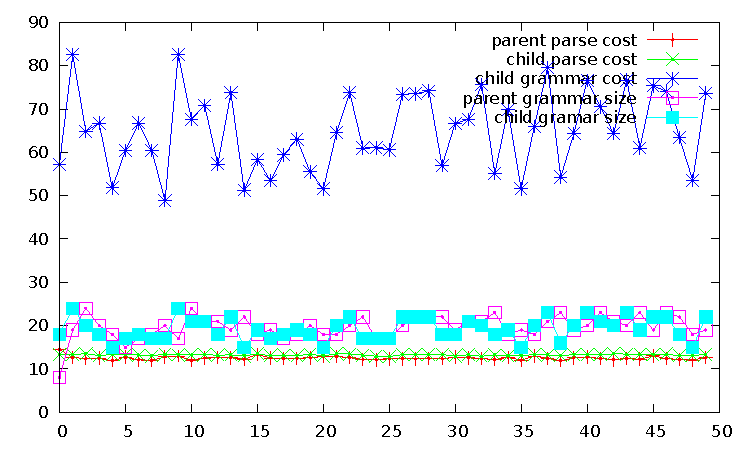
\includegraphics[width=\textwidth]{debug_10_50_0_1_F_F_stat.pdf}
                \caption{}
                \label{fig:costsA}
        \end{subfigure}%
        ~ %add desired spacing between images, e. g. ~, \quad, \qquad etc.
          %(or a blank line to force the subfigure onto a new line)
        \begin{subfigure}[b]{0.3\textwidth}
                \centering
                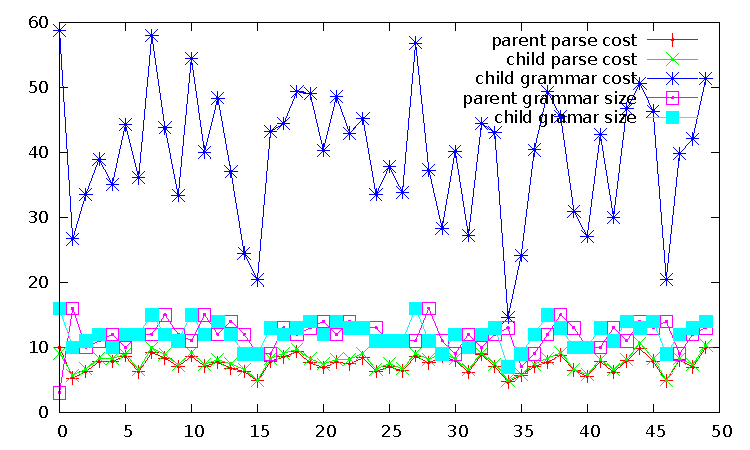
\includegraphics[width=\textwidth]{debug_10_50_0_1_T_F_stat.pdf}
                \caption{}
                \label{fig:costsB}
        \end{subfigure}
        ~ %add desired spacing between images, e. g. ~, \quad, \qquad etc.
          %(or a blank line to force the subfigure onto a new line)
        \begin{subfigure}[b]{0.3\textwidth}
                \centering
                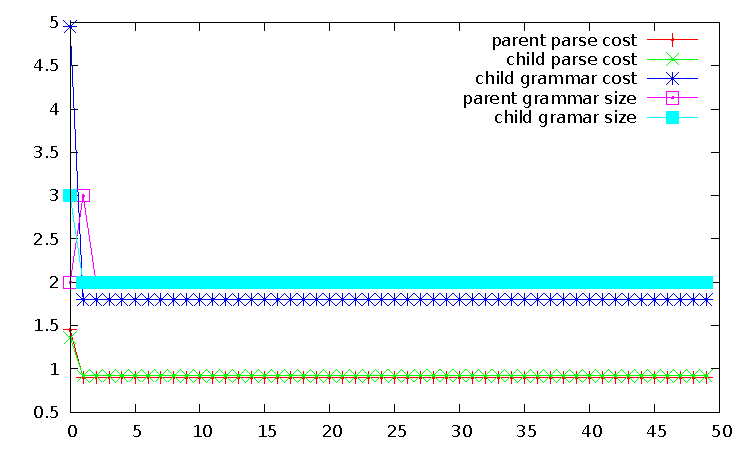
\includegraphics[width=\textwidth]{debug_10_50_0_1_T_T_stat.pdf}
                \caption{}
                \label{fig:costsC}
        \end{subfigure}

% exploration rate = 0.1
        \begin{subfigure}[b]{0.3\textwidth}
                \centering
                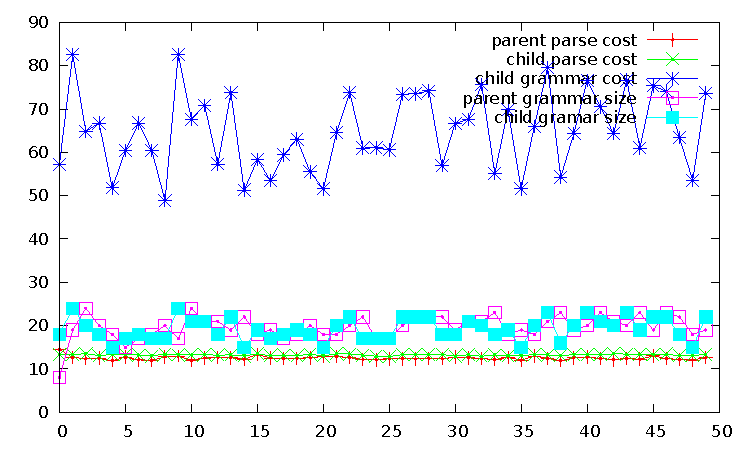
\includegraphics[width=\textwidth]{debug_10_50_01_1_F_F_stat.pdf}
                \caption{}
                \label{fig:costsD}
        \end{subfigure}%
        ~ %add desired spacing between images, e. g. ~, \quad, \qquad etc.
          %(or a blank line to force the subfigure onto a new line)
        \begin{subfigure}[b]{0.3\textwidth}
                \centering
                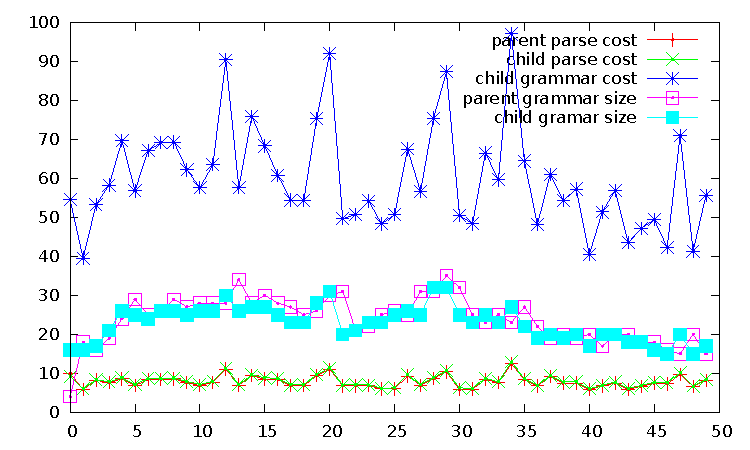
\includegraphics[width=\textwidth]{debug_10_50_01_1_T_F_stat.pdf}
                \caption{}
                \label{fig:costsE}
        \end{subfigure}
        ~ %add desired spacing between images, e. g. ~, \quad, \qquad etc.
          %(or a blank line to force the subfigure onto a new line)
        \begin{subfigure}[b]{0.3\textwidth}
                \centering
                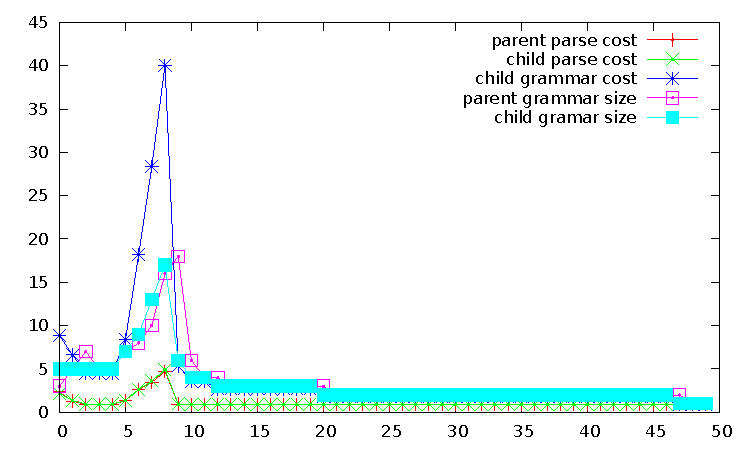
\includegraphics[width=\textwidth]{debug_10_50_01_1_T_T_stat.pdf}
                \caption{}
                \label{fig:costsF}
        \end{subfigure}

% exploration rate = 0.5
        \begin{subfigure}[b]{0.3\textwidth}
                \centering
                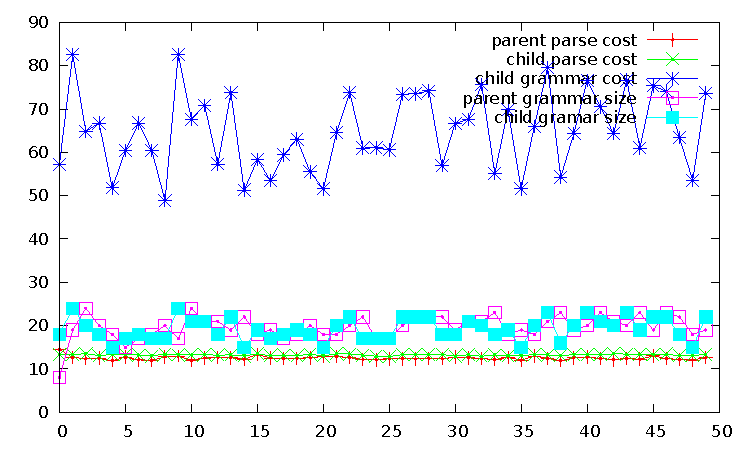
\includegraphics[width=\textwidth]{debug_10_50_05_1_F_F_stat.pdf}
                \caption{}
                \label{fig:costsG}
        \end{subfigure}%
        ~ %add desired spacing between images, e. g. ~, \quad, \qquad etc.
          %(or a blank line to force the subfigure onto a new line)
        \begin{subfigure}[b]{0.3\textwidth}
                \centering
                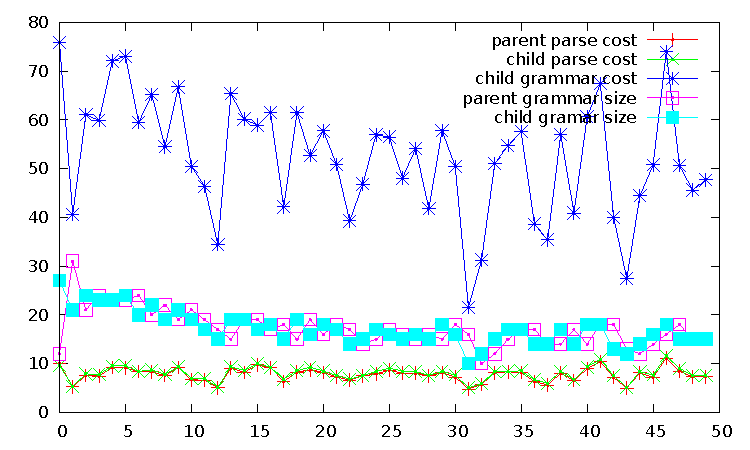
\includegraphics[width=\textwidth]{debug_10_50_05_1_T_F_stat.pdf}
                \caption{}
                \label{fig:costsH}
        \end{subfigure}
        ~ %add desired spacing between images, e. g. ~, \quad, \qquad etc.
          %(or a blank line to force the subfigure onto a new line)
        \begin{subfigure}[b]{0.3\textwidth}
                \centering
                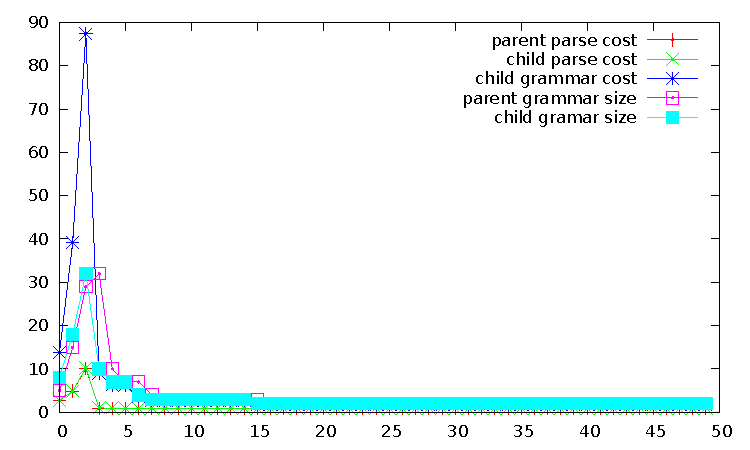
\includegraphics[width=\textwidth]{debug_10_50_05_1_T_T_stat.pdf}
                \caption{}
                \label{fig:costsI}
        \end{subfigure}

% exploration rate = 1.0
        \begin{subfigure}[b]{0.3\textwidth}
                \centering
                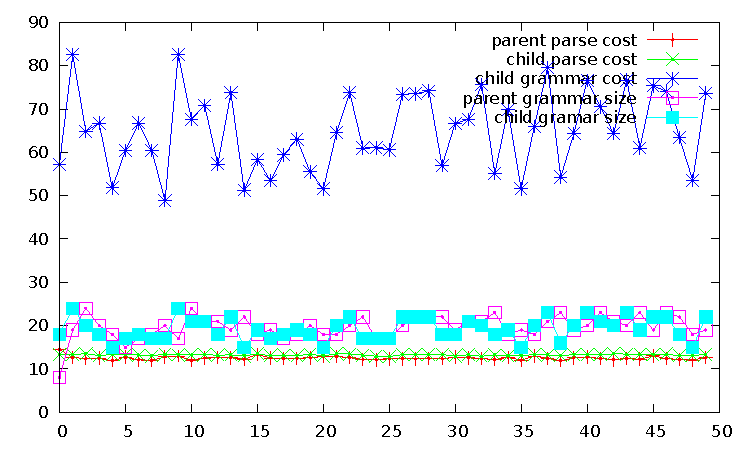
\includegraphics[width=\textwidth]{debug_10_50_1_1_F_F_stat.pdf}
                \caption{}
                \label{fig:costsJ}
        \end{subfigure}%
        ~ %add desired spacing between images, e. g. ~, \quad, \qquad etc.
          %(or a blank line to force the subfigure onto a new line)
        \begin{subfigure}[b]{0.3\textwidth}
                \centering
                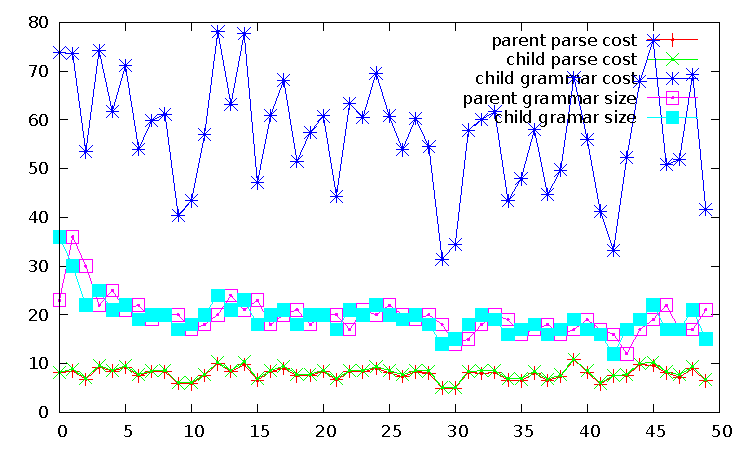
\includegraphics[width=\textwidth]{debug_10_50_1_1_T_F_stat.pdf}
                \caption{}
                \label{fig:costsK}
        \end{subfigure}
        ~ %add desired spacing between images, e. g. ~, \quad, \qquad etc.
          %(or a blank line to force the subfigure onto a new line)
        \begin{subfigure}[b]{0.3\textwidth}
                \centering
                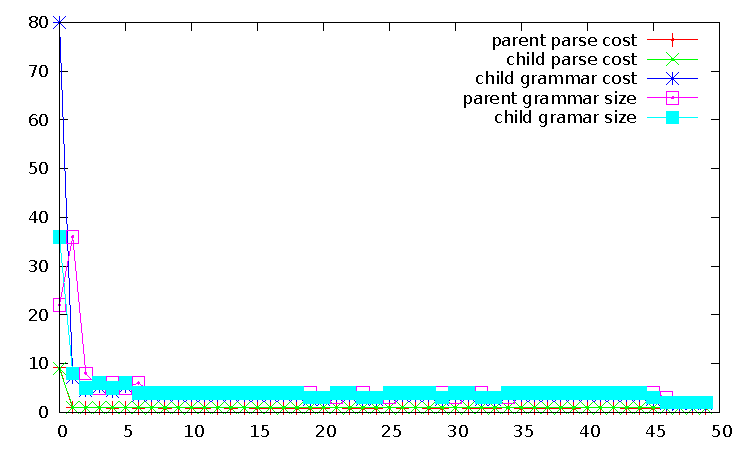
\includegraphics[width=\textwidth]{debug_10_50_1_1_T_T_stat.pdf}
                \caption{}
                \label{fig:costsL}
        \end{subfigure}

        \caption{Each figure shows the parent's average parse cost (red), the child's average parse cost (green), the parent's grammar size (pink), the child's grammar size (cyan) and the child's grammar cost (blue) for each iteration. The figures in the first, second and third column use uniform sampling, predicate sampling and template sampling, respectively. The four rows correspond to the exploration rates $\langle 0.0, 0.1, 0.5, 1.0 \rangle$.}
        \label{fig:costs}
\end{figure}

\section{Results}
\label{sec:results}
The third column in figure \ref{fig:costs} shows that sampling both templates and predicates from the grammar (see section \ref{ssec:Template sampling}) causes the grammar size to quickly converge which produces only intentions with one formula. This is to be expected, since this sampling approach is analogous to the sampling of strings in \cite{zuidema2003poverty}, i.e. the parent's sampled intentions are fully conditioned on its grammar.

The first column shows the other end of the spectrum: sampling intentions uniformly from a fixed set. The parent will always be likely to verbalize intentions that are not in its grammar, which means the language can never be too small. The iterative process does not produce a structured grammar, because the intentions produced by the parent are not dependent of the grammar it has learned when it was a child\footnote{Since sampling is not dependent of the grammar and each simulation used the same seed, all 4 plots show the same results.}. This can again be seen in the high cost of the child's grammar. After learning certain intentions as a child, in the next iteration it is just as likely to produce cheap intentions using the rules of its grammar as it is to produce expensive new intentions.

Finally, we have chosen a middle ground (second column in figure \ref{fig:costs}) where the template of an intention is sampled uniformly but the the content of the intention is sampled conditioned on the parent's grammar. This sampling approach ensures the grammar remains expressive while at the same time favors intentions that can be constructed by the grammar. We expected an iterated effect would occur, in which the child's grammar cost would gradually decrease over time. That, however, did not happen. The figures in the second column show a lower cost for the child's grammar compared to the first column, but experience more fluctuations. This is caused by the fact a child is more likely to send the observations it receives once it becomes a parent, which reduces the child's grammar cost. However, if the parent sends a lot of intentions that are unknown to the child, the child's grammar suddenly increases and all the progress made in previous iterations is lost.

The different exploration rates do not account for much difference in the results when applied to uniform sampling or predicate sampling. With template sampling, the exploration rate denotes how quickly the iterative process converges. Figure \ref{fig:costsI} ($\epsilon = 0.5$) has a higher exploration rate than figure \ref{fig:costsF} ($\epsilon = 0.1$), which means that the iterative process in figure \ref{fig:costsI} is likely to find a cheap intention to communicate quicker than the process in figure \ref{fig:costsF} and thus converge faster. Figure \ref{fig:costsC} has an exploration rate $\epsilon = 0.0$, which means the parent will not sample new intentions after is has sampled the first one. Figure \ref{fig:costsL} ($\epsilon = 1.0$), on the other hand, continuously samples new intentions. 

\section{Discussion}
\label{sec:discussion}
The results with the predicate sampling technique did not show evidence for the grammar becoming increasingly structured and cheaper to learn over time. We believe the explanation for this is that the intentions received by a child during one iteration does not have enough influence on the intentions that are constructed in the next iteration. Uniform sampling of templates could cause so much variation that the amount of information that is transmitted from parent to child is too small. This can be solved by either reducing the amount of templates which can be sampled or by increasing the amount of intentions that are communicated per iteration.

A big difference between the context-free rules discussed in this paper and the context-free rules used in \cite{zuidema2003poverty} is that the left-hand-side of one of our rules is not an abstraction of its right-hand-side but its union. This means our grammar is not a true context-free-grammar, but instead is mildly context-sensitive. It would be interesting to see the effect of using abstract semantic categories on the left-hand-side of rules. Figure \ref{fig:abstraction} shows an example of a derivation with abstracted intentions: \textit{tweety} and \textit{pussycat} are substituted by the intentions \textit{bird} and \textit{cat}, respectively. Each step in the derivation the intentions become more abstract until a unique intention \textit{I} is reached that covers the whole sentence. This approach, however, would greatly complicate the problem of iterated learning, since clustering would need to be performed in order to form abstract intentions and know which intentions should be substituted by this abstract intention.

\begin{figure}[h!]
\centering
\Tree [.\text{I} [.\text{[(object, 1), (action, 1, 2), (object, 2)]} [.\text{[(bird, 1)]} [.\text{[(tweety, 1)]} tweety ]] [.\text{[(saw, 1, 2), (cat, 2)]} [.\text{[(saw, 1, 2)]} saw ] [.\text{[(pussycat, 2)]} pussycat ]]]]
\caption{A derivation with abstracted intentions}
\label{fig:abstraction}
\end{figure}

\section{Conclusion}
\label{sec:conclusion}


\bibliographystyle{plainnat}
\bibliography{references}

\end{document}
